\chapter{Seizure Prediction}

Electroencephalograms(EEG) capture the electromagnetic 
potential of similarly aligned neurons firing in unison. Although a number of correlations between 
EEG and physiological phenomena have been found the relation between EEG and neural circuitry dynamics are still not well-understood \cite{eeg}. 
one difficulty is relating in vitro behavior of individual neural cells with in vivo behavior of both local and global neural dynamics.  
For a neuropathological condition like epilepsy, 
the challenge is to relate global spread of 
synchronized firing to local cellular mechanisms.

In this chapter, we analyze EEG data gathered 
from a group of mice afflicted with a genetic 
mutation that causes early onset epilepsy similar to 
Dravet syndrome. This was an exploratory study to assess how well stimulus-induced seizures could be predicted and to find those features correlated with the likelihood of a seizure. 

The study of complex biological signals like EEG 
was one of the motivations for developing the 
$\varepsilon-$complexity feature. EEG are non-stationary
signals that exhibit transient waveforms and apparent regime changes over relatively short periods of times. In the context of dynamical systems, a regime change describes an alternation between semi-stable states 
\cite{lorenz2006}. While we do not assume the brain dynamics can be described as a non-linear dynamical system, the term is useful for characterizing the
observed behavior of EEG signals. 

A common method of analyzing EEG is to compute some set of features on the raw signal and use averages of the features over fixed windows. The procedure 
serves as a way of reducing the high-dimensional 
EEG signal and extracting a more interpretable
feature set. One drawback of this method is that the process of averaging over arbitrary windows may obscure important features associated with the varying dynamics of the brain. 

Previous studies have used a change-point detection algorithm applied to the raw EEG signal 
to segment and cluster these varying brain states, 
for example, the sleep states of neo-nates\cite{pirya2009}.
The $\varepsilon-$complexity feature is meant to capture an intrinsic feature of the signal. As shown in 
Chapter 4, the feature may also be related to the 
fractal dimension of a signal which Gneiting describes
as a second order statistical property of 
a signal through its relation to the variogram or 
correlation function\cite{gneiting2012}. 

In this chapter, we design a classifier that modifies
the typical feature extraction method segmenting the signal based on the $\varepsilon-$complexity coefficients. 
We compare classification accuracy on a dynamically segmented
set of features to several models that uniformly segment the feature set. For each of these models, we 
attempt to predict seizures based on features 
extracted from individual EEG channels rather than from the full set of six. The set of EEG channels correspond to specific functional regions of the brain.  
Feature extraction and classification based on individual channels allows us to make more fine-grained inferences about the combination of feature and region that are associated with a seizure response.


% The $\varepsilon-$complexity feature was develope with 

% The ECoG -- which I will refer to simply as EEG --
% signal captures changes in field potential caused by large 
% groups of aligned neurons firing synchronously. The LFP sensors
% capture a signal from a smaller cluster of neurons.

% a way to detect changes in the underlying dynamics that generate some signal. Specifically, the analysis of EEG was a motivating test case. EEG signals measure changes in 
% electrical potential generally at the outer layer or cortex of the brain. 

% \section{Seizure Prediction}


\section{EEG Data}

The EEG data gathered from 4 mice with a genetic 
mutation in the voltage-gated sodium channel gene Scn1a 
a similar mutation to that causing Dravet syndrome 
The mutation results in early onset epileptic seizures \cite{ito2013}.
The mice were equipped with 4 electrocortical(ECoG) sensors --intracranial sensors placed directly on the brain cortex --  
along with 2 local field potential (LFP) sensors located 
 in the thalamus.  
The mice were genetically modified to produce a light sensitive protein, an opsin, allowing for direct stimulation of neurons with a laser pulse train. 

% \begin{figure}[!htbp]
%   \begin{center}
%   % \begin{picture}(60,60)
%   % ./figs/coeff-interp-simple-functions1.pdf
%   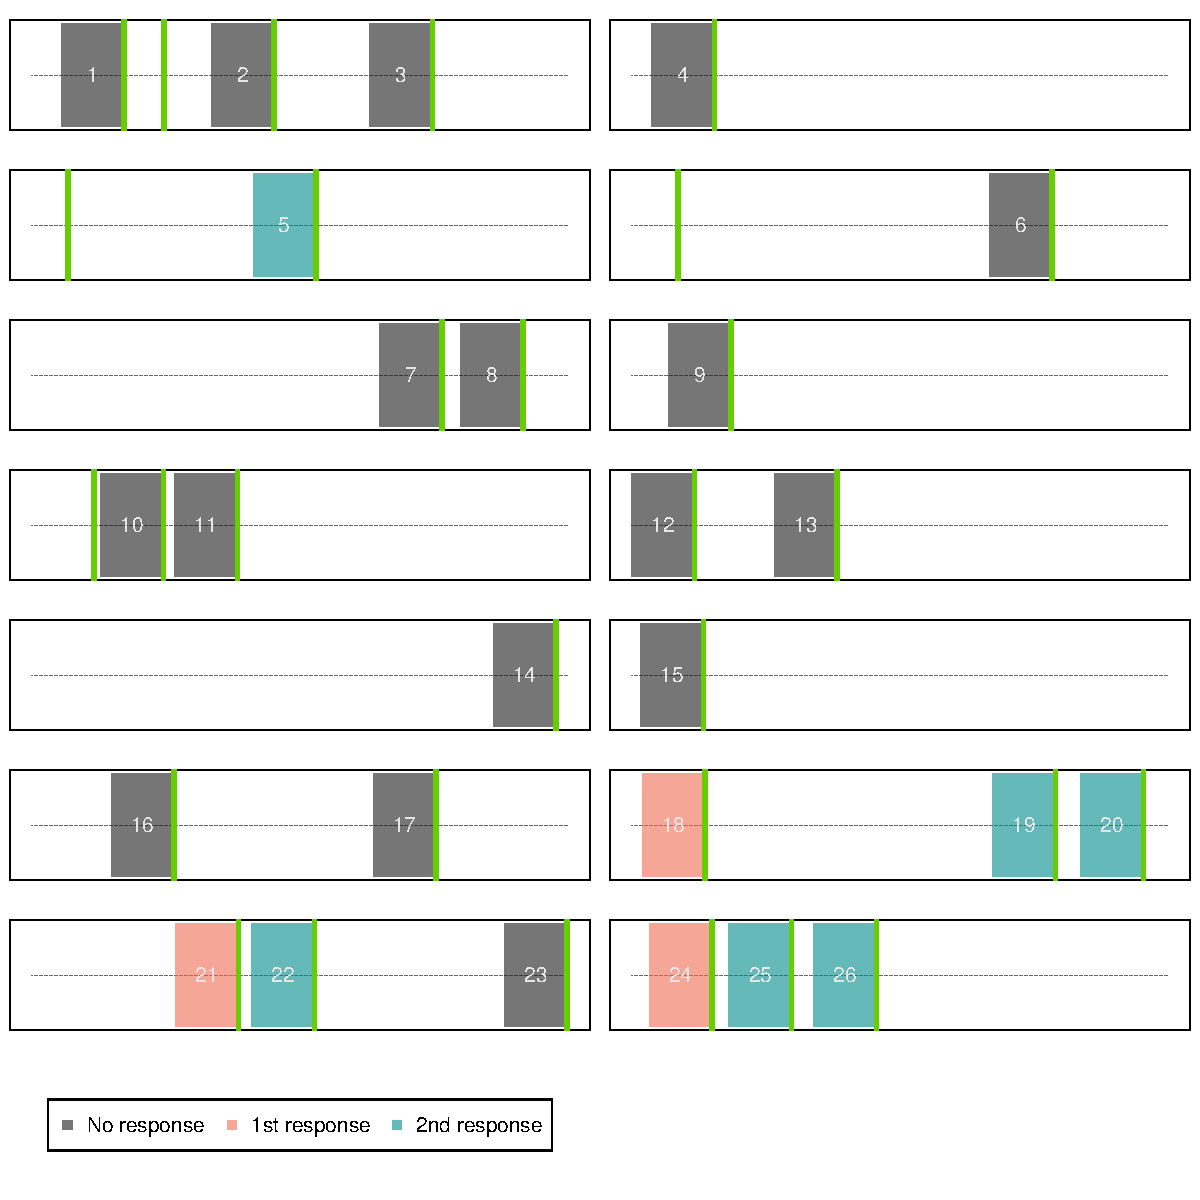
\includegraphics[width = \textwidth, keepaspectratio]{./figs/trialplot.pdf}
%   % \end{picture}
%   \end{center}
%   \label{fig:trialplot} 
%   \caption{Schematic plot of trial data. Each rectangle 
%            represents a single time period. The green 
%            vertical bars indicate applications of the stimulus.}
% \end{figure}

Data was gathered from 13 distinct time periods during which the was applied one to four times. 
4-minute segments preceding the stimulus were used as the final set of 26 trials. The results of each 
trial was were coded as either a seizure, which 
we refer to as a positive response, or no seizure. 
Coding was based on the visible response of the 
mouse. The EEG signals around the stimulus period were also visually examined to check the accuracy of the coding.

The EEG was sampled at 1220.7 Hz and
a bandpass filter removed frequencies below 0.5 Hz and greater
than 300 Hz. A notch filter was applied at 60 Hz and its harmonic frequencies. 


\section{EEG Features}
We selected a feature set consisting of standard 
spectral characteristics along with a few additional 
features. The power in frequency bands 
delta, theta, alpha, beta, and gamma was calculated 
as the integral of the spectral density $f(\lambda)$ 
computed as a smoothed periodogram. For example, 
delta band power, $\delta B$, corresponds to 
the frequency band $0.5-4Hz$ and integrates  
$f(\lambda)$ over over this interval
\[
  \B = \int_{0.5}^{4} f(\lambda) d\lambda. 
\]
The frequency bins corresponding to the remaining bands are, 
in order,$ 4-8Hz, 8-12Hz, 12-30Hz, 30-100Hz$. 

Additional features were selected based on two tests.
A set of non-linear features including sample entropy,
and permutation entropy, spectral entropy, a Hurst 
parameter estimator and fractal dimension along with wavelet coefficients  and variance were tested for their ability to discriminate between the same two groups of simulations used in Chapter 3 to test the approximation methods used in estimating complexity coefficients. Based on these results, spectral entropy, fractal dimension, the Hurst parameter and the wavelet coefficients, along with the spectral band power features and the complexity coefficients were computed on the EEG. In informal testing
with a baseline classification model, the wavelet coefficients did not improve classification results and were removed from the final feature set. Given more data, feature selection might have been better performed through cross-validation on a training set. On the other hand, one of our goals was to work with a reduced feature set that was more readily interpretable. 

We have defined most of the features used in classification in Chapter 2. Spectral Entropy is a measure of the distribution in the spectrum of a signal. 
\[  
  SE = - \int_{-\pi}^{\pi} f_x(\lambda) \log f(\lambda) d \lambda.
\]
The Hurst parameter was estimated using the corrected empirical Hurst exponent\cite{weron2002}.  
 
All features were calculated on non-overlapping 2-second intervals. The final list of feature used in classification was 
\begin{enumerate}
\item Delta, theta, alpha, beta, gamma 
\item Spectral entropy 
\item Hurst parameter
\item Variance
\end{enumerate}

The complexity coefficients were used in our segmentation 
classifier but not as a feature. The variogram estimator of fractal dimension, $\hat D$ was also computed but was omitted from the final models as the feature appeared closely correlated with the complexity coefficient $B$. 

% Figure \ref{fig:trialplot}
% is a schematic picture of the trial periods. 
% There are several trials that did not follow a previous 
% seizure, and below we compare whether the features
% for these trials appear to come from a distribution 
% similar to the seizure response trials that followed 
% a previous seizure.

% Segmentation on the complexity coefficients is a 
% depends on the 
% Initially, the features were computed on 4 second intervals but at this resolution no change points were detec

\section{Segment Classifier}

% Although raw EEG time series values are used in some classification approaches, when using neural-network based classifiers for example,
%  a common approach is to compute a set of features on the time series and use 
% these features as predictors. Using features rather than raw time series 
% serves to reduce the dimensionality of the data. 
Whether it is spectral features or $\varepsilon-$complexity 
features, the mapping of the raw data to the 
features results both in a dimensionality 
reduction and an averaging over some variation and structure 
in the data. That is, there is a trade-off between losing 
important variation in the data and reducing the dimension
of the raw input. In our approach, we compute features 
in three basic steps. Features are computed at a relatively 
fine resolution for each EEG channel. Given an 
individual channel, the time series formed by the features
is segmented based on changes in the complexity coefficients. 
The weighted averages of the features set on these segments is
used as a training set for the classifier. 


% We selected a small set of features for our classifier. 
% These included the band power of the  
% frequency bands delta, theta, alpha, beta and. 
% Spectral features need 
% to be computed over a windowed section of the time series 
% that is some multiple of the lowest frequency being computed 
% in order for the power estimates to have some statistical 
% validity. So using spectral features inherently reduces 
% the dimensionality of the data, for example, from several 
% thousand points a set of six values representing the 
% band power of some window of frequencies will be computed. 
%  Features including the 
% complexity coefficients are computed on 2 second intervals. 
% Change-points in the complexity coefficients are then 
% used to segment the features. The final predictor 
% is the mean of the features computed on each segment.
% The basic steps used are outlined below.

 %   \begin{algorithm}[!htbp]
 %    \label{alg:segmenet}
 %  \caption{Single channel segment classifier \label{alg:ecomplex}}
 %  \DontPrintSemicolon
 %  \SetAlgoLined
 %  \SetKwInOut{Input}{Input}\SetKwInOut{Output}{Output}
 %  \Input{$ \mathcal{F} $ a set of multivariate time series
 %      $\textbf{f} $ corresponding of length $N$.}
 %  \Input{$\mathcal{L}_f$ a set of labels $l_f$ for each time series 
 %  $ \textbf{f} $ }
 %  \Input{$\mathcal{X}$ a set of time series $x_f$ of length $N$ 
 %  used to partition each $\textbf{f}$.} 
 %  \Output{$\mathcal{M}$ a trained classification model.}
 %  % \tcp{initialize array}
 %   % Initialize the array epsilons $\leftarrow [0]$   \;
 %  \BlankLine 
 % \ForEach{$f$ in $\mathcal {F}$} {    
 %    % \tcp{initialize array}    
 %   Compute the change points for $\mathcal{x}_f$
 %      $p_f \leftarrow$  change_pts($\mathcal{X}_f$)
 %   Segment $f$ on change points $x_f$
 %     $\{ f \} \leftarrow f$
 %    \ForEach{$f$ in $\mathcal{F}$} {
 %      % \tcp{Compute the approximation error}
 %        Compute the approximation error \\ 
 %        $\varepsilon_{h,f} \leftarrow 
 %       \frac{1}{N}\norm{f_h - X_{h} }^2$.  \;
 %      % mse\leftarrow \varepsilon_{h,f}$
 %    } 
 %     Find minimium error over all $f$  \\
 %     epsilons$_h$ $\leftarrow \min \varepsilon_{h,f}$. \;
 %  }
 %  Fit a least squares linear model \\
 %   $A,B$ $\leftarrow$ lm(epsilons$_h$ $ \sim \{ \mathbb{S}_h \} $.) \;
 %  \end{algorithm}

\begin{enumerate}
  \item For each channel compute set of features
        on regular intervals including 
        $\varepsilon-$complexity.
  \item For each channel, compute the change points 
        in $\varepsilon-$complexity. 
  \item For each trial, segment all features using the change point 
        set computed in the previous step. 
  \item Compute the mean of each feature on the 
        segments. 
   \item Label the means of the segments 
         in a training 
         set with the label of the full time 
         series and use this set to train 
         a classifier.
   \item Train a classifier on the means of the 
         segments. 
  \item  For the means of the segmented test set,
         compute the class probability of each 
       segment using the trained 
         classifier. 
  \item  For each trial use the prediction probabilities of each segment weighted by segment length to compute the final class probability.
\end{enumerate} \label{alg:segment-alg}

In the case of a uniform partition of the features, this
the method is equivalent to simply using the average class probability for each segment to classify the trial.

In theory, any classifier, or several classifiers could be used in steps 5 and 6. We used a random forest classifier. The random forest is constructed from a large number of individual decision trees. For numeric data, the decision trees partition the feature space into $d-$dimensional rectangles each labeled with a class. The decision trees branches correspond to partitions of the feature space. For each branch, a subset of the features are chosen and the split is made in order to increase the class purity of each partition. The final prediction is based on the combined vote of the individual trees.  In addition to random selection of features, a random subset of observations are used to build each tree. This allows for an out-of-bag(OOB) estimate of the classifier 
accuracy which is calculated by classifying each observations using the set of trees which were built without seeing that observation \cite{breiman2001}.

\begin{figure}[!htbp]
  \begin{center}
  % \begin{picture}(60,60)
  % ./figs/coeff-interp-simple-functions1.pdf
  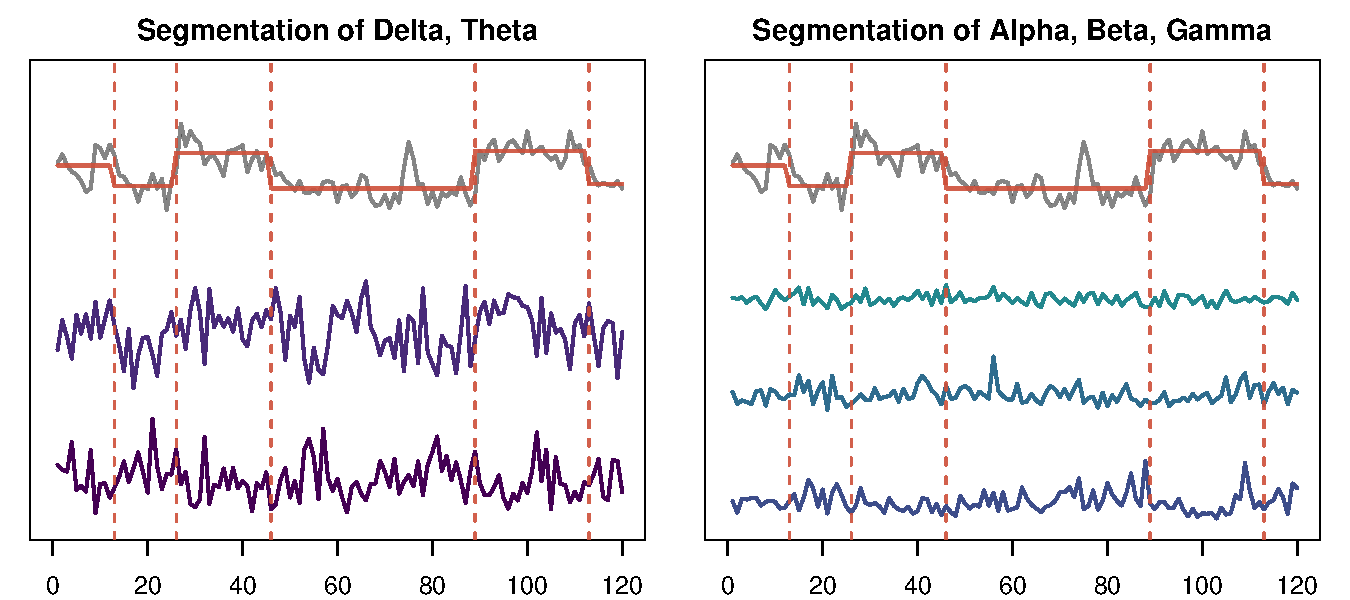
\includegraphics[width = \textwidth, keepaspectratio]{./figs/eeg-segment-plot.pdf}
  % \end{picture}
  \end{center}
  \label{fig:segplot} 
  \caption{Spectral features segmented on changes in the B complexity coefficient.}
\end{figure}

\section{Model Performance}

We begin by defining several terms we will be using to describe classifier performance. We term a seizure a 
positive response or simply a response. A  
\textit{true positive}  
is an accurate prediction of a seizure while a 
 \textit{true negative} is an accurate prediction of a non-response. 
The  \textit{sensitivity} of the classifier is then 
defined as the proportion of true positives to total 
positive and  \textit{specificity} is the total of true 
negatives to total negatives. We use the term accuracy to refer to balanced accuracy
\[
  \text{Balanced Accuracy} = \frac{\text{Sensitivity + Specificity}}{2}.
\] 
We also report AUC, or area under the ROC curve, see 
Figure \ref{fig:eegroc} for an example from two 
of the classifiers tested. The 'curve' is the plot 
of the sensitivty against the false positive rate or 
$1 - $specificity and a higher AUC indicates a better performing classifier.

We created a simple baseline classification model to compare to the segmented classifiers. The feature set for this model was the mean of each of the 8 features on the six channel resulting in 48 features. A random forest classifier was trained on these features and the out-of-bag classification results are reported in table \ref{tab:baseline}.

% Asymptotically this is an unbiased estimate the error on a

 \begin{table}[!htbp] \centering 
 
\begin{tabular}{@{\extracolsep{5pt}} cccc} 
\\[-1.8ex]\hline 
\hline \\[-1.8ex] 
 & Sensitivity & Specificity & Accuracy \\ 
\hline \\[-1.8ex] 
1 & $0.544$ & $0.935$ & $0.740$ \\ 
\hline \\[-1.8ex] 
\end{tabular} 
 \caption{Classification performance of baseline classifier.} 
  \label{tab:baseline} 
\end{table} 


% \begin{table}[!htbp]
% \begin{center}
%   \begin{tabular}{ | c | c |  c|} 
%   \hline 
%  Sensitivity & Specificity  &  Accuracy  \\ \hhline{|=|=|=|}
%   0.54  &  0.94     &    0.74  \\ \hline
% \end{tabular}  
% \caption{Prediction performance for baseline classifier.}
% \label{tab:baseline}
% \end{center}
% \end{table}

We compared six models to this baseline model. For each 
model a different partition scheme was used. For the models
using complexity coefficients we denote $A, B, A+B$ where 
each trial was partitioned based 
on change points detected in the corresponding complexity 
coefficients and the $A + B$ model is simply the union 
of the change points of both complexity coefficients. 
Three other models used regular partitions.   
Each trial was uniformly segmented into $8, 15$ or $30$ segments and we refer
to these models by the partition number. 

The performance of these models was assessed using 
5-fold cross-validation where balanced sets were used for the hold-out set for each fold. The reported results are based on 10 repetitions or bootstrap samples. Results for a larger number of repetitions, 50, were similar. We report to smaller sample to emphasize the relative sizes of the confidence intervals of the reported performance measures. In general, all models performed best on the LFP channels, 
here labeled channel 1 and 2. These sensors are located in the thalamus and measure the electrical potential of a small set of neurons. The best performing model was the regularly partitioned model with 8 segments followed by the model $A+B$.

\begin{figure}[!htbp]
  \begin{center}
  % \begin{picture}(60,60)
  % ./figs/coeff-interp-simple-functions1.pdf
  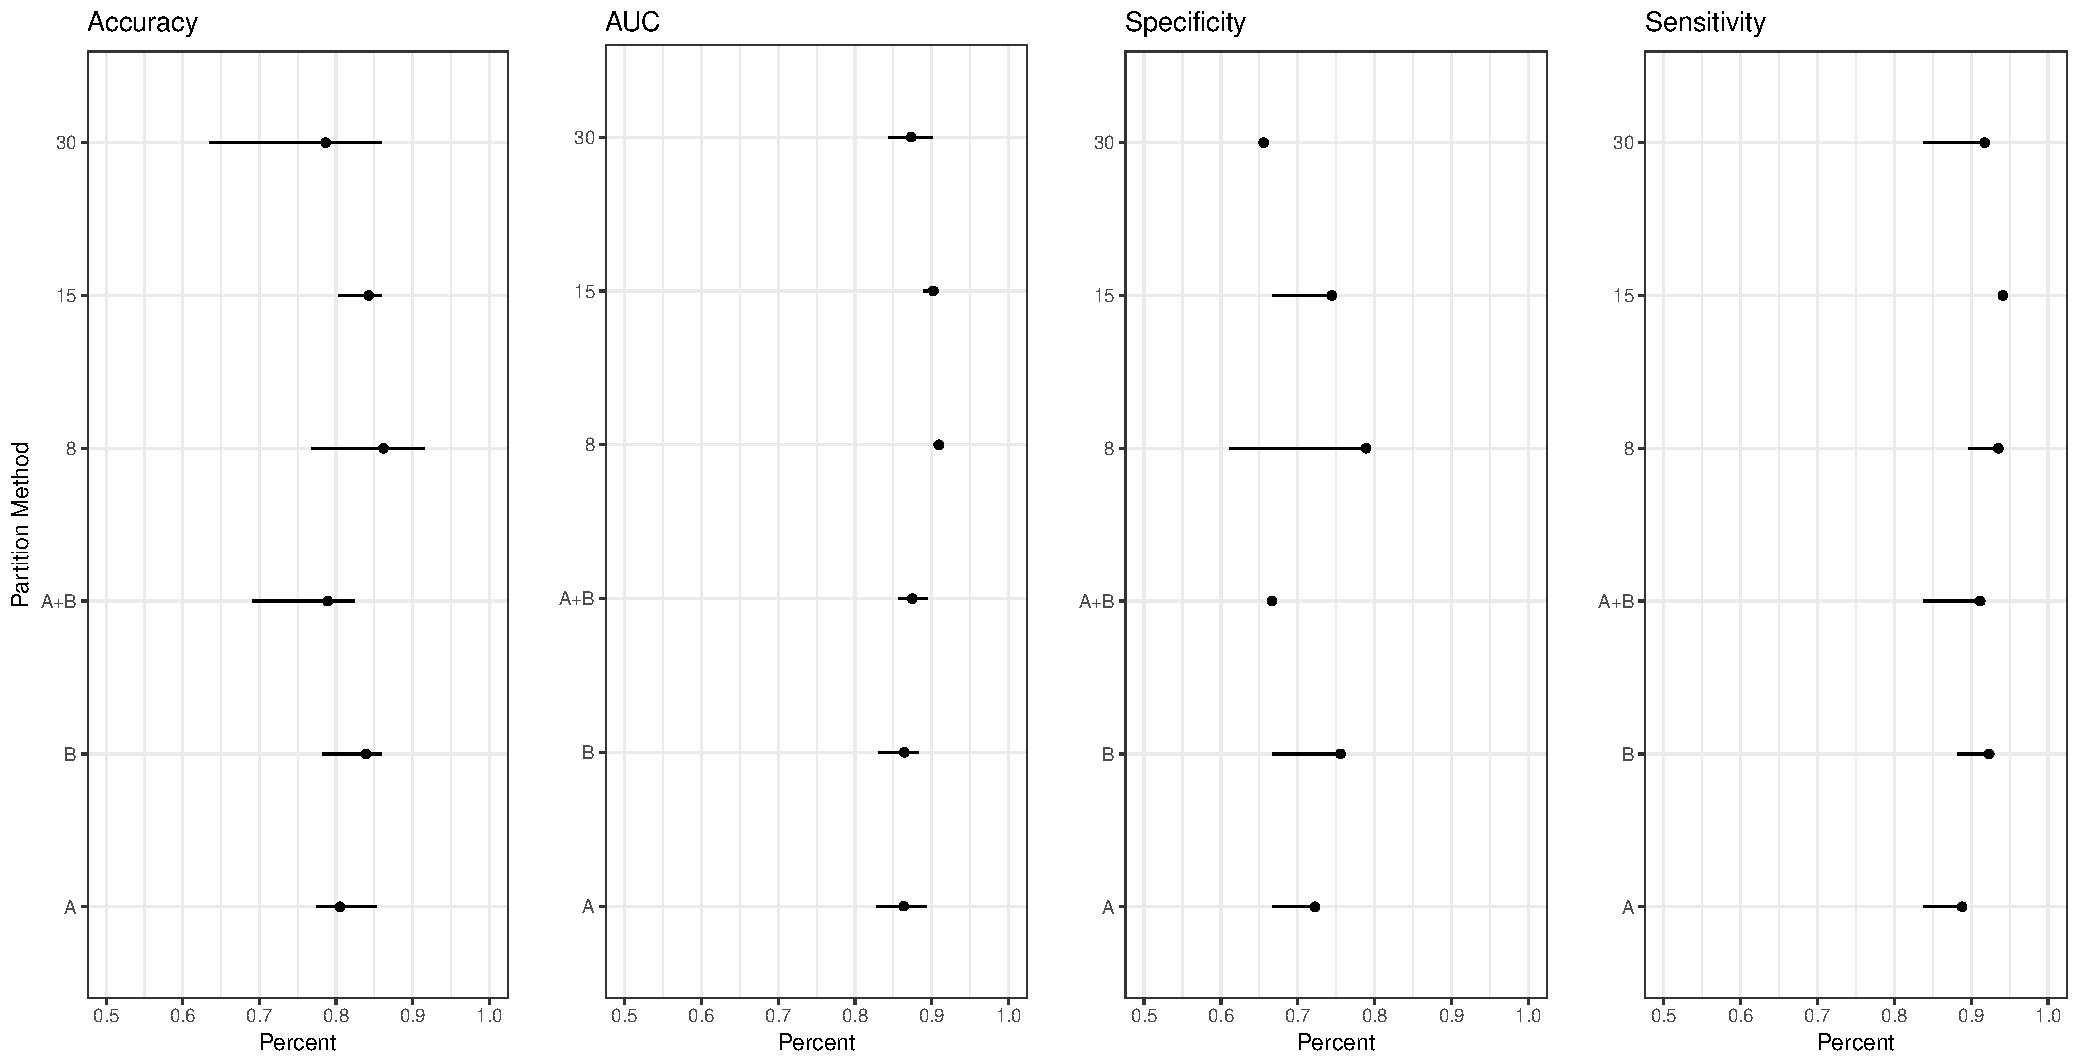
\includegraphics[width = \textwidth, keepaspectratio]{./figs/eeg-partition-diagnostic.pdf}
  % \end{picture}
  \end{center}
  \caption{Classification diagnostic values for each partition method for LFP channel 1.}
  \label{fig:eeg-diagnostic} 
\end{figure}

The performance measures for each classifier on channel 
1 are shown in figure \ref{fig:eeg-diagnostic}. The 
mean and 95\% confidence interval based on 10 
bootstrap classifications are reported.  All methods classified 
non-response trials well but the two better performing
 models -- model 8  and model $A+B$ -- 
had relatively high accuracy in classifying seizure responses: 76\% for model $A+B$ and 79\% for model 8. 

Classification is generally more difficult 
when classes are unbalanced, that is, when there are 
significantly fewer observations in the training 
set of one class compared to the other. Other 
than performing cross-validation on a balanced 
hold-out set, no other adjustments were made in 
the underlying random forest model or the 
threshold probability for selecting a class.  

% \begin{minipage}{0.45\textwidth}
\begin{table}[!htbp] \centering 
\begin{tabular}{@{\extracolsep{1pt}} ccccccc} 
\\[-1.8ex]\hline 
\hline \\[-1.8ex] 
 & Ch1 & Ch2 & Ch3 & Ch4 & Ch5 & Ch6 \\ 
\hline \\[-1.8ex] 
A & $0.76$ & $0.76$ & $0.70$ & $0.71$ & $0.57$ & $0.60$ \\ 
B & $0.78$ & $0.77$ & $0.70$ & $0.69$ & $0.60$ & $0.64$ \\ 
A+B & $0.84$ & $0.70$ & $0.69$ & $0.71$ & $0.59$ & $0.61$ \\ 
8 & $0.85$ & $0.81$ & $0.69$ & $0.71$ & $0.68$ & $0.82$ \\ 
15 & $0.79$ & $0.79$ & $0.73$ & $0.71$ & $0.73$ & $0.73$ \\ 
30 & $0.78$ & $0.80$ & $0.72$ & $0.71$ & $0.72$ & $0.84$ \\ 
\hline \\[-1.8ex] 
\end{tabular} 
  \caption{Balanced accuracy for each model and channel} 
  \label{tab:all-accuracy} 
\end{table} 
% \end{minipage}
% \hfill

% \begin{minipage}{0.45\textwidth}
\begin{table}[!htbp] \centering  
\begin{tabular}{@{\extracolsep{1pt}} ccccccc} 
\\[-1.8ex]\hline 
\hline \\[-1.8ex] 
 & Ch1 & Ch2 & Ch3 & Ch4 & Ch5 & Ch6 \\ 
\hline \\[-1.8ex] 
A & $0.64$ & $0.58$ & $0.46$ & $0.49$ & $0.23$ & $0.28$ \\ 
B & $0.66$ & $0.59$ & $0.48$ & $0.53$ & $0.36$ & $0.34$ \\ 
A+B & $0.76$ & $0.46$ & $0.46$ & $0.52$ & $0.28$ & $0.30$ \\ 
8 & $0.79$ & $0.68$ & $0.48$ & $0.51$ & $0.50$ & $0.69$ \\ 
15 & $0.69$ & $0.63$ & $0.52$ & $0.50$ & $0.62$ & $0.53$ \\ 
30 & $0.62$ & $0.67$ & $0.51$ & $0.49$ & $0.57$ & $0.76$ \\ 
\hline \\[-1.8ex] 
\end{tabular} 
  \caption{Specificity for all models and channels.} 
  \label{tab:specificity}
\end{table} 
% \end{minipage}

The balanced accuracy all models for each channel is shown in Table \ref{tab:all-accuracy}. All partition
schemes resulted in fairly high rates of accuracy for channels 1 and 2. The models with a higher number of 
partitions performed significantly better on the 
ECoG channels 3-6. On the other hand, accurate classification of seizures tailed off sharply for all ECoG channels as seen in Table \ref{tab:specificity}. 

\begin{figure}[!htbp]
  \begin{center}
  % \begin{picture}(60,60)
  % ./figs/coeff-interp-simple-functions1.pdf
  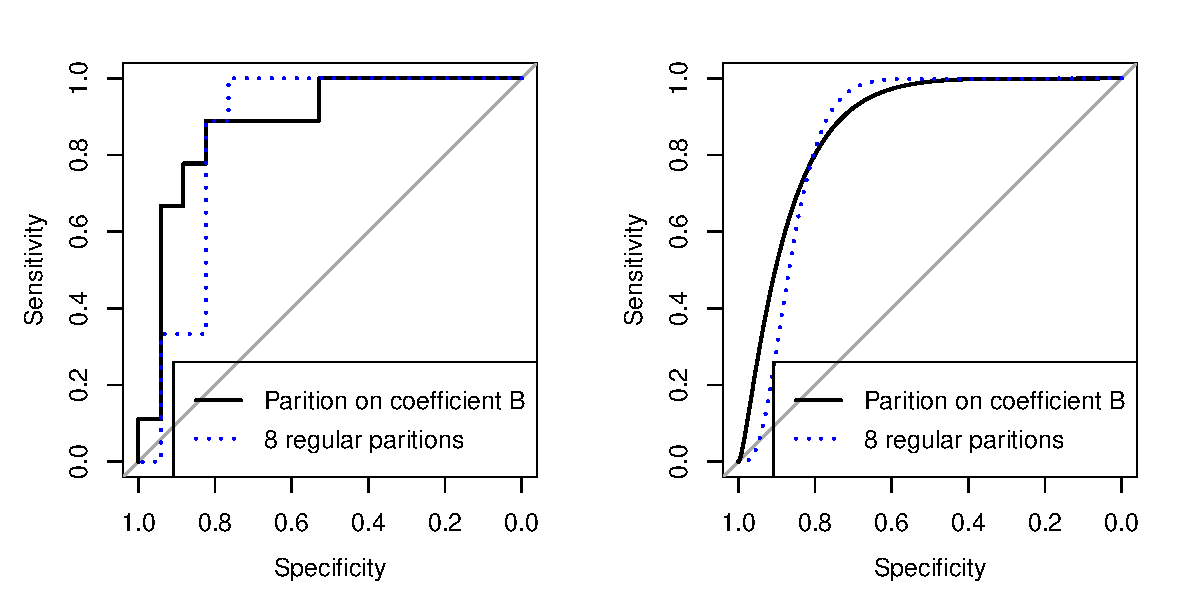
\includegraphics[width = \textwidth, keepaspectratio]{./figs/eegroc-comb.pdf}
  % \end{picture}
  \end{center}
  \caption{ROC curves and smoothed ROC curves
           for classification on channel 1 using 
           partitions on coefficient B and a regular partition into 
           8 segments.}
\end{figure}
\label{fig:eegroc} 
\section{Feature Importance}

As mentioned above, with only a small set of observations, 
improved classification on one or two instances
would affect the performance of the classifier.
Whether the model used here --
partitions based on complexity coefficients -- would be successful in other contexts remains to be seen. 
One of our assumptions was that arbitrary partitioning would average over changes variations in the features that corresponded to transient states. 
But whether the complexity coefficients capture significant
changes in the underlying dynamics that are useful for classfication might depend on both feature selection and the classification task. 

% \begin{table}[!htbp]
% \begin{center}
%   \begin{tabular}{ | c | c |  c| c | c | c |c| } 
%   \hline 
% Channel       &     1&    2 &    3 &     4 &     5 &    6  \\ \hline
% Partition Type    &       &      &     &     &  &  \\ \hhline{|=|=|=|=|=|=|=|}
% A    & 0.81 & 0.78 & 0.69 & 0.72  & 0.57  & 0.63  \\ \hline
% B    & 0.84 & 0.77 & 0.72 & 0.70  & 0.57  & 0.65  \\ \hline
% A+B  & 0.81 & 0.74 & 0.73 & 0.72  & 0.55  & 0.60  \\ \hline
% 8    & 0.86 & 0.84 & 0.73 & 0.72  & 0.74  & 0.75  \\ \hline
% 15   & 0.85 & 0.81 & 0.74 & 0.73  & 0.75  & 0.75  \\ \hline
% 30   & 0.79 & 0.75 & 0.76 & 0.77  & 0.72  & 0.77  \\ \hline
%       \end{tabular}  
% \caption{Balanced classification accuracy for each partition method 
%          and each channel.}
% \label{tab:error-allch}
% \end{center}
% \end{table}

% Table created by stargazer v.5.2 by Marek Hlavac, Harvard University. E-mail: hlavac at fas.harvard.edu
% Date and time: Sun, Jun 25, 2017 - 10:27:00 PM
 
A goal of our study was to determine features  
predictive of seizures. The selection of a reduced
the feature set and prediction on isolated channels
allow us to measure the feature importance for 
classification for each sensor location.
The distributions of features for response and non-response trials are looked
at below. Examining the one-dimensional distribution of the feature may not reveal interactions between the features in higher dimensions. 
On the other hand, decision trees divide up the feature space in complex ways and the final ensemble votes are what determines the classification outcome. 
In theory, those features found to be useful in classification will not necessarily be identifiable with basic summary statistics such as the mean, median or variance. However, for our data, the features used by the best predictors were associated with significant distributional differences across classes.
%  in particular 
% the features trained on predictors trained on the LFP channels 1 and 2. 

\begin{figure}[h]
  \begin{subfigure}[b]{0.45\textwidth}
      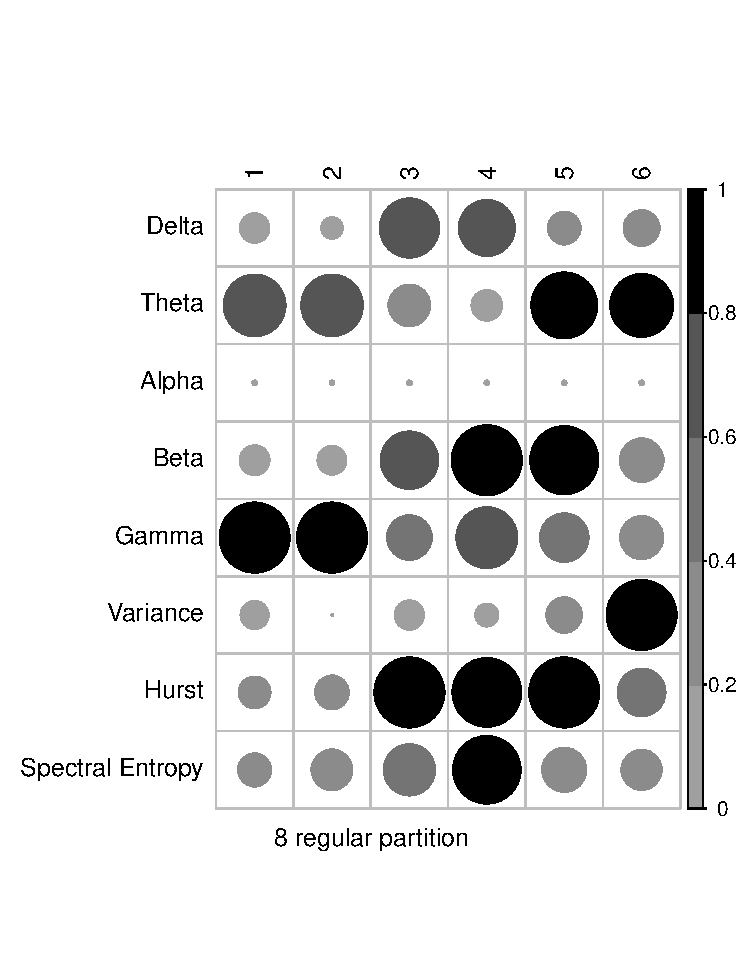
\includegraphics[width = \linewidth, keepaspectratio]{./figs/eeg-vec-corrplot.pdf}% \end{picture}
    % \caption{Functions without added noise.}
    % \label{fig:corrplot}
  \end{subfigure} 
  \hfill
  \begin{subfigure}[b]{0.45\textwidth}
    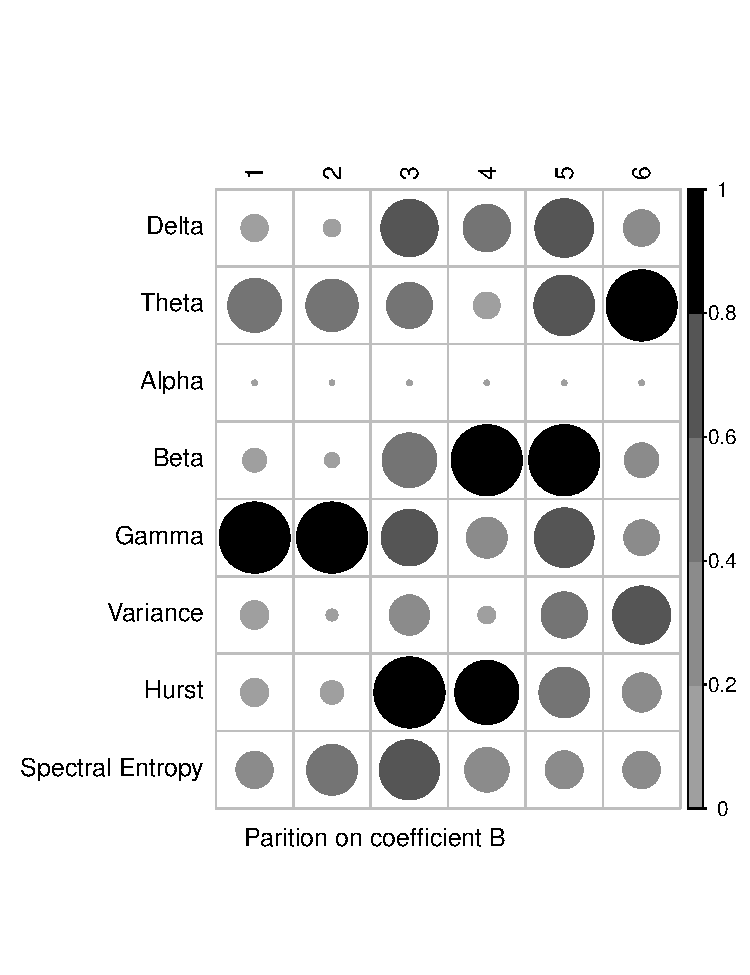
\includegraphics[width = \linewidth, keepaspectratio]{./figs/eeg-AB-corrplot.pdf}% \end{picture}
  % 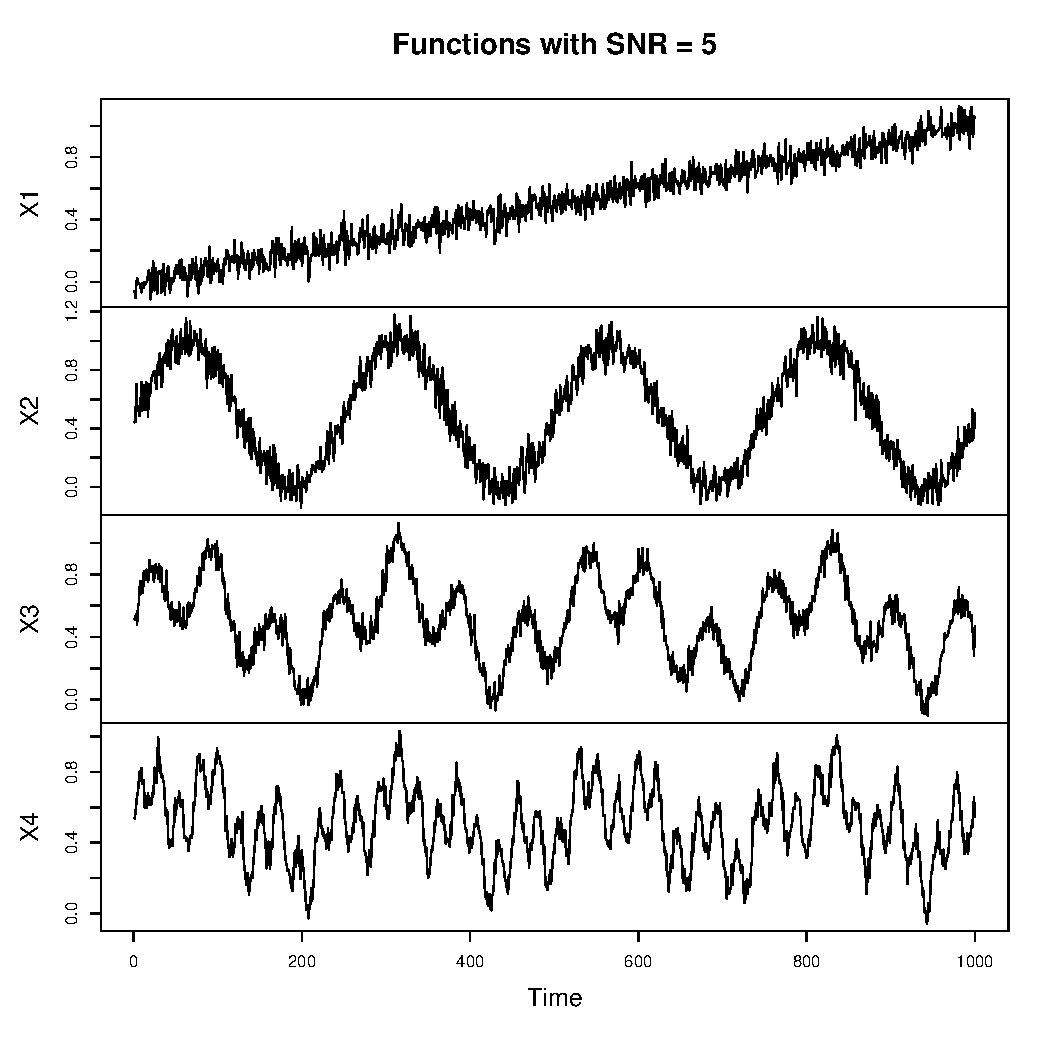
\includegraphics[width = 0.9\linewidth, height = 3in]{./figs/coeff-interp-simple-functions1.pdf}
    % \caption{Functions without added noise.}
      \end{subfigure}
  \caption{Variable importance for
   partition methods normalized to 
  a $[0,1]$ interval for each channel.}
    \label{fig:corrplot}
\end{figure}

We report the mean variable importance of the random forest classifiers trained during cross-validation. Variable importance is determined by the mean decrease in the
class Gini index when branches are made on a given feature
\cite{breiman2001}. Informally, variable importance
measures how well a feature divides response trials from non-response
trials. In Figure \ref{fig:corrplot} we show the variable 
importance for the two best performing models $A+B$ and the 
model $8$. We have normalized variable importance to a $[0,1]$ interval for each model and
channel so the figure shows the relative importance of the variable for each model. There is a common pattern in the variable importance across the two models. Gamma and theta bands have the highest importance for the best performing models, those trained on the LFP channels 1 and 2. 
Both partition methods also show increased importance for beta on channels 4 and 5 and increase the importance of the Hurst coefficient for channels 3 and 4. 

\begin{figure}[!htbp]
  \begin{subfigure}[b]{ \textwidth}
  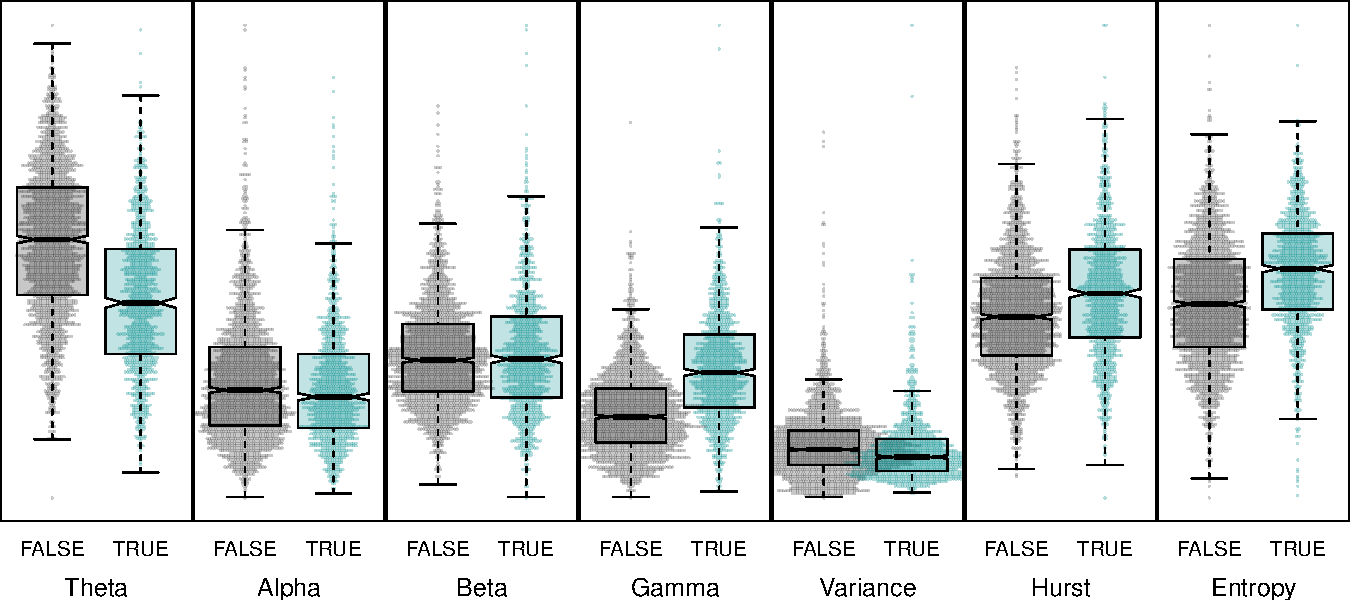
\includegraphics[width = \textwidth, keepaspectratio]{./figs/eeg-boxplot1.pdf}
    % \label{fig:corrplot}
  \end{subfigure} 
  \hfill
  \begin{subfigure}[b]{\textwidth}
  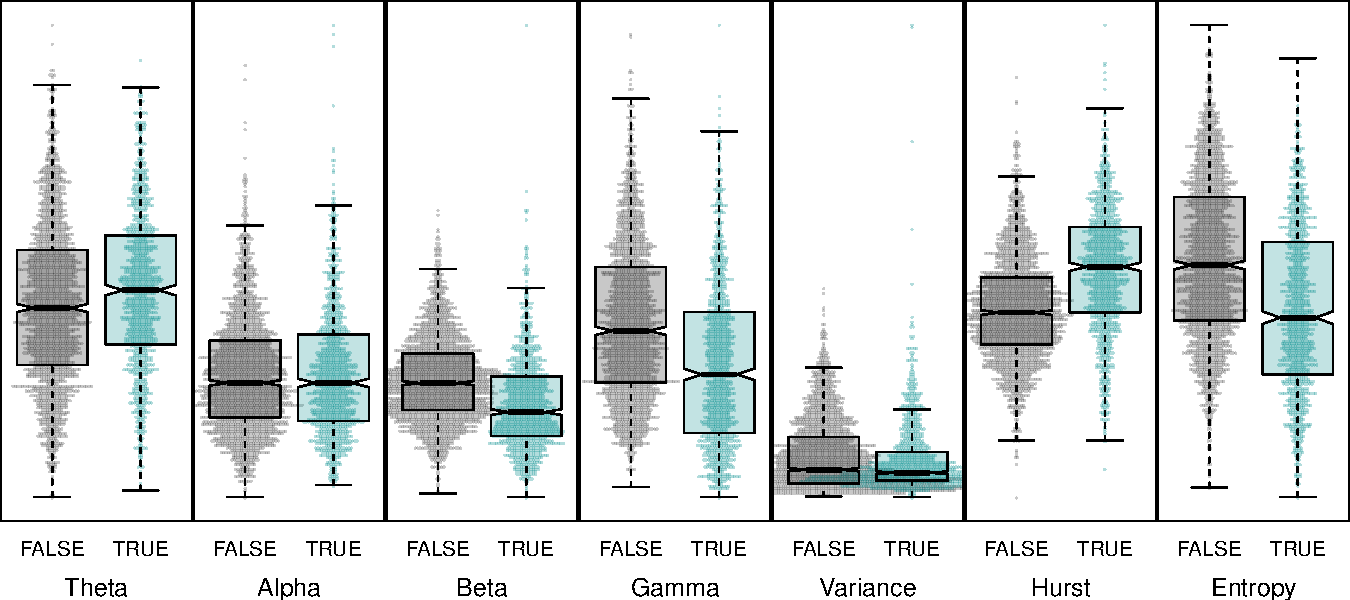
\includegraphics[width = \textwidth, keepaspectratio]{./figs/eeg-boxplotch3.pdf}
  % 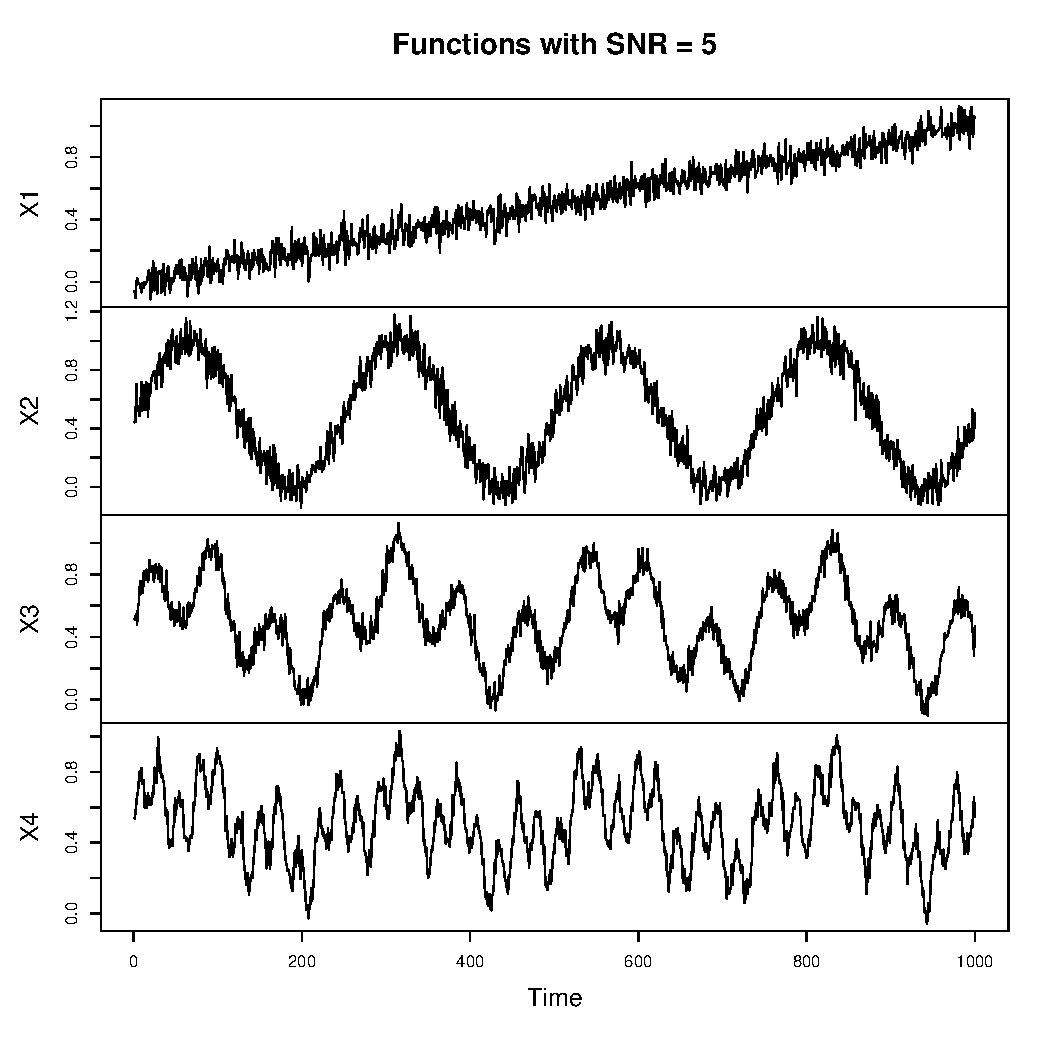
\includegraphics[width = 0.9\linewidth, height = 3in]{./figs/coeff-interp-simple-functions1.pdf}
    % \caption{Functions without added noise.}
      \end{subfigure}
  \caption{Feature distribution for channels 1 and 3.}
  \label{fig:boxplot}
\end{figure}

% \begin{figure}[!htbp]
%   \begin{center}
%   % \begin{picture}(60,60)
%   % ./figs/coeff-interp-simple-functions1.pdf
%   % \end{picture}
%   \end{center}
%   \label{fig:eegroc} 
%   \caption{Feature distribution for channel 1.}
% \end{figure}

% \begin{figure}[!htbp]
%   \begin{center}
%   % \begin{picture}(60,60)
%   % ./figs/coeff-interp-simple-functions1.pdf
%   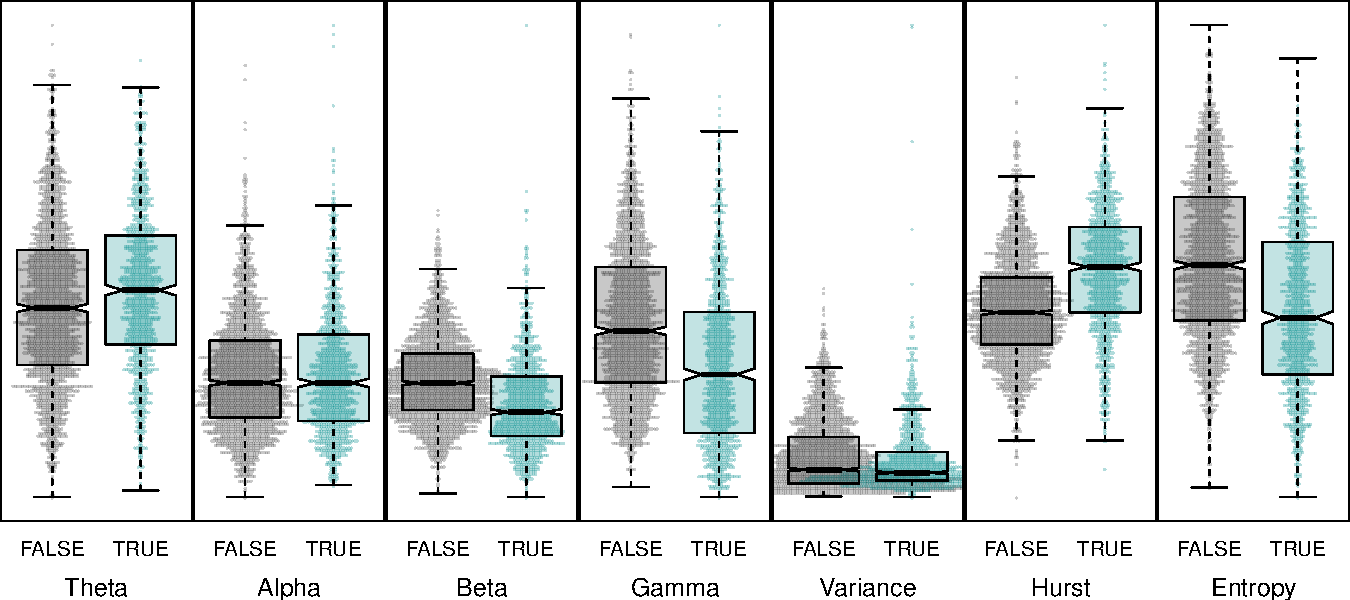
\includegraphics[width = \textwidth, keepaspectratio]{./figs/eeg-boxplotch3.pdf}
%   % \end{picture}
%   \end{center}
%   \label{fig:eegroc} 
%   \caption{Feature distribution for channel 1.}
% \end{figure}

Variable importance as measured by the random forest classifiers 
was also reflected in distributional differences in the features. 
The boxplots in figure \ref{fig:boxplot} show the distribution 
and features for channels 1 and 3.  For channel 1, the relative 
power of gamma is higher and theta lower for trials with 
seizure responses. The median of theta and gamma fall outside the inter-quartile range and a similar distribution was similar for channel two.  For channel three, the relative power of theta
and gamma are reversed with gamma lower and theta higher. 
On the other hand, the distribution of beta for channels 1 and 2 
were similar while beta was significantly lower for channels 3 and 4. Table \ref{tab:pvals}
shows the p-value determined by the Wilcox rank-sum test. While a large number of data points guarantees that even small differences will be statistically significant, the table does highlight the non-significant values. 


% Table created by stargazer v.5.2 by Marek Hlavac, Harvard University. E-mail: hlavac at fas.harvard.edu
% Date and time: Mon, Jun 26, 2017 - 08:05:44 PM

\begin{table}[!ht] \centering 
\begin{tabular}{@{\extracolsep{5pt}} ccccccc} 
\\[-1.8ex]\hline 
\hline \\[-1.8ex] 
 Channel & 1 &  2 &  3 &  4 & 5 &  6 \\ 
\hline \\[-1.8ex] 
Delta & $< .0001$ & $< .0001$ & $< .0001$ & $< .0001$ & $< .0001$ & $< .0001$ \\ 
Theta & $< .0001$ & $< .0001$ & $< .0001$ & $< .0001$ & $< .0001$ & $< .0001$ \\ 
Alpha & $0.022$ & $0.699$ & $0.897$ & $0.891$ & $0.008$ & $0.302$ \\ 
Beta & $0.826$ & $0.226$ & $< .0001$ & $< .0001$ & $< .0001$ & $< .0001$ \\ 
Gamma & $< .0001$ & $< .0001$ & $< .0001$ & $< .0001$ & $< .0001$ & $< .0001$ \\ 
Variance & $< .0001$ & $< .0001$ & $0.687$ & $0.005$ & $< .0001$ & $< .0001$ \\ 
Hurst & $< .0001$ & $< .0001$ & $< .0001$ & $< .0001$ & $< .0001$ & $< .0001$ \\ 
Spectral Entropy & $< .0001$ & $< .0001$ & $< .0001$ & $< .0001$ & $0.0003$ & $< .0001$ \\ 
\hline \\[-1.8ex] 
\end{tabular} 
  \caption{Wilcox rank sum test p-values for difference of medians.} 
  \label{tab:pvals} 
\end{table} 

\section{Discussion} 

While we were able to predict a seizure result 
with relatively high accuracy using several 
classification methods, there are some 
limitations to the study. Several mice 
were used in the experiments but the 
trials resulting in seizures came from a single mouse. 
Additional data from other mice would be needed 
to know whether the results reported here generalize. 
In addition, most of the seizures 
came from stimuli applied within two trials. This means
several seizures occured after a previous seizure. 
The features found predictive of a seizure may  
be conflated with features that are a result of a seizure. 
% As mentioned in the limitations section, the seizure responses 
% came in all cases from a single mouse and most of those 
% seizures came in trial periods during which there was more than one 
% seizure. Whether the predictive model generalizes to other cases
% and whether the differences in features that were predictive of 
% a seizure are similar for other subjects remains open. 
Because of the small number of trials, we did not 
have a hold-out data set. The lab from which produced this 
set of data is currently collecting additional data which will 
enable us to test how well the predictive models generalize 
and whether the observed differences in features hold for other 
subjects. 

% Although feature importance seemed robust to changes 
% in the partitions comparing feature performance across other 
% predictive models 
The segmentation model based on the complexity coefficients performed as well or somewhat better than two of the models with regular partitions. However, the regular partition models tended to perform more consistently across channels and the partition model with 8 segments outperformed the models segmented on the complexity coefficients. All models classified negative responses well so differences in model performance were based
mostly on the classification of seizure responses of which there were only 9. The partition based on complexity coefficients is based on a change point algorithm which is somewhat sensitive to the number of data points. Using an increased number of data points, 
for example, by taking measurements on an overlapping sliding window rather than on non-overlapping windows, may reduce the variability in how a time series is segmented based on the complexity coefficients. Tests of the model on simulated data sets or a wider range of time series would be needed to assess the performance of the model in more general contexts. 








